\documentclass[10pt]{article}
\usepackage[letterpaper,text={6.5in,8.7in},centering]{geometry}
\usepackage{amssymb,amsmath,times,url,subfigure,graphicx,multirow}
\usepackage[pdftex,urlcolor=blue,pdfpagemode=none,pdfstartview=FitH]{hyperref}
\usepackage[final]{pdfpages}
\usepackage{biblatex}
\addbibresource{library.bib}
%% url smaller font.
\makeatletter
\def\url@leostyle{%
  \@ifundefined{selectfont}{\def\UrlFont{\sf}}{\def\UrlFont{\small\ttfamily}}}
\makeatother
\urlstyle{leo}

%\usepackage[all,import]{xy}


\renewcommand{\baselinestretch}{1.2}
\date{}

\renewcommand{\thesubsection}{\arabic{subsection}. }
\renewcommand{\thesubsubsection}{\arabic{subsection}.\arabic{subsubsection} }


\begin{document}
\pagestyle{empty}
\section*{MAE 3145: Orbital Mechanics \& Space Dynamics}
\vspace*{-0.4cm}
\noindent{Fall 2018, W 1810--2040, SEH 3040}

%From 2012, Delete Chapter 5, and revise the course calendar.

\paragraph*{Instructor}
Shankar Kulumani\quad Email: \href{mailto:skulumani@gwu.edu}{skulumani@gwu.edu}\quad Homepage: \url{http://fdcl.seas.gwu.edu/}\\
\hspace*{1.8cm}
Office Hour: TBD 


\paragraph*{Prerequisites} APSC 2058 Analytical Mechanics II

\paragraph*{Course Description} This course covers the motion of spacecraft under gravity. Included are the derivation and the analyses of the two-body problem and their applications for real world missions.
Extensive use of scientific programming languages is required to simulate orbital dynamics and solve real-world astrodynamics problems.

\paragraph*{Textbook}
\begin{list}{$\bullet$}{\setlength{\itemsep}{-3pt}}
\item R. Bate, \textit{Fundamentals of Astrodynamics}, Dover Publication, 1971
\end{list}


\paragraph*{Contents}
\begin{list}{$\bullet$}{\setlength{\itemsep}{-3pt}}
\item Astrodynamic Fundamentals
    \begin{list}{$-$}{\setlength{\itemsep}{-3pt}}
    \item Time [BMW Chap. 2.9]
    \item Coordinate Systems [ BMW Chap. 7.4]
    \item Project RV2COE
    \end{list}
\item Orbital Mechanics\vspace*{-0.2cm}
    \begin{list}{$-$}{\setlength{\itemsep}{-3pt}}
    \item Dynamics of Point Masses [Curtis Chap. 1]
    \item Two-Body Problem [ BMW Chap. 1]
    \item Orbital Elements [ BMW Chap. 2.3]
    \item Groundtracks [ BMW Chap. 2.15]
    \item Project COMFIX
    \item Project PROPOGATE
    \end{list}
%\item Orbit Determination\vspace*{-0.2cm}
%    \begin{list}{$-$}{\setlength{\itemsep}{-3pt}}
%    \item Gibbs Method [Chap. 5]
%    \end{list}
\item Orbital Maneuvers\vspace*{-0.2cm}
    \begin{list}{$-$}{\setlength{\itemsep}{-3pt}}
    \item Hohmann Transfers [ BMW Chap. 3]
    \item Plane Changes [ BMW Chap. 3.4]
    \item Orbital Rendezvous and Phasing [ BMW Chap. 8.3]
    \end{list}
\item Perturbations
    \begin{list}{$-$}{\setlength{\itemsep}{-3pt}}
    \item Geopotential []
    \item Drag
    \item PREDICT
    \end{list}
\end{list}

\paragraph*{Software Projects}
A major focus of this course will be the application of sound scientific programming skills.
You will apply the theoretical tools of astrodynamics to solve realistic problems by implementing your own library of tools.

\begin{list}{$\bullet$}{\setlength{\itemsep}{-3pt}}
    \item RV2COE - convert position and velocity vectors of a spacecraft to classical orbital elements
    \item COMFIX - determine the orbital elements of a satellite given ground based radar observations
    \item PROPOGATE - determine the position of a satellite as a function of time
    \item PREDICT - predict satellite passes for any location on the Earth
    \end{list}
\paragraph*{Additional Readings - Other sources of useful information}
\begin{list}
{$\bullet$}
{\setlength{\itemsep}{-3pt}}
\item \fullcite{vallado2007}
\item \fullcite{battin1999}
\item J. Danby, \textit{Fundamentals of Celestial Mechanics}, Willmann-Bell, 1988
\item J. Prussing, \textit{Orbital Mechanics}, Oxford University Press, 1993
\item V. Chobotov, \textit{Orbital Mechanics}, AIAA, 2002
\item T. Logsdon, \textit{Orbital Mechanics: Theory and Applications}, Wiley, 1997
%%\item R. Dorf, and R. Bishop, \textit{Modern Control Systems}, Prentice Hall, 2007
%\item K. Ogata, \textit{Modern Control Engineering}, Prentice Hall, 2001
%\item N. Leonard and W. Levine, \textit{Using MATLAB to Analyze and Design Control Systems}, Addison Wesley, 1995
\item Scipy Tutorial: \href{http://www.scipy-lectures.org/}{http://www.scipy-lectures.org/}
\end{list}
%\renewcommand{\thesubfigure}{}
%\begin{figure}[h]\vspace*{-0.3cm}
%\centerline{
%\subfigure[Etkin]{
%    \href{http://books.google.com/books?id=AIIOAAAACAAJ}%
%    {\includegraphics[height=2.3cm]{etkin.pdf}}}
%\subfigure[Nelson]{
%    \href{http://books.google.com/books?id=bt46AAAACAAJ}%
%    {\includegraphics[height=2.3cm]{nelson.jpg}}}
%\hspace*{0.5cm}
%\subfigure[Stevens]{
%    \href{http://books.google.com/books?id=T0Ux6av4btIC}%
%    {\includegraphics[height=2.3cm]{stevens.jpg}}}
%\subfigure[Stengel]{
%    \href{http://books.google.com/books?id=nI_EHQAACAAJ&dq=stengel+flight&ei=YpKkSL7tL4L2iQG7hZ36BA}%
%    {\includegraphics[height=2.3cm]{stengel.jpg}}}
%\subfigure[Roskam]{
%    \href{https://oscommerce.darcorp.com/product_info.php?cPath=21&products_id=125&osCsid=077f051b037aa4a35b9b6e52998bbae8}%
%    {\includegraphics[height=2.3cm]{roskam.jpg}}}
%\hspace*{0.5cm}
%\subfigure[Anderson]{
%    \href{http://books.google.com/books?id=Hd_AR0CAmsoC}%
%    {\includegraphics[height=2.3cm]{anderson.jpg}}}
%\subfigure[McClamroch]{
%    \href{http://my.fit.edu/~taeyoung/McClamroch.pdf}%
%    {\includegraphics[height=2.3cm]{nhm.pdf}}}}
%\end{figure}

\paragraph*{Grading}
Homework 35\%,\;\; Attendance 5\%,\;\; Midterm Exam 20\% ,\;\; Final Exam 20\%, \;\; Projects 20\%


\paragraph*{Course Learning Objectives}
At the end of this course, students will be able to:

\newcounter{lcounter}
\begin{list}
{\arabic{lcounter}:}
{\setlength{\itemsep}{-3pt}\usecounter{lcounter}}
\item Explain the Newtonian gravitational force and gravitational potential between particles
%\item Understand the dynamics of a system of two particles acting under their mutual gravitational potential
\item Analyze the characteristics of circular, elliptic, parabolic and hyperbolic orbits in a two-dimensional plane
\item Describe the geometry of an orbit in a three-dimensional space from orbital elements
\item Apply numerical/analytical techniques to propogate orbits.
\item Choose and apply the approprite orbital maneuvering method to move spacecraft between orbits.
\item Develop personal software tools to solve practical astrodynamic problems:
    \begin{itemize}
        \item Determine orbital parameters from ground based observations.
        \item Predict satellite passes and determine observation angles to view satellites overhead.
    \end{itemize}
\end{list}


\paragraph*{ Minimum out of class work per week}
\begin{itemize}
    \item Direct Instruction - 2.5 hours
    \item Indendent Learning - 5 hours
\end{itemize}

\newpage
\paragraph*{General Policy}
\begin{list}
{\arabic{lcounter}:}
{\setlength{\itemsep}{-3pt}\usecounter{lcounter}}

\item \textbf{Check your GW email account daily}. All of the important announcements of this class will be made through Blackboard/email. 

\item All work must follow  The George Washington University Code of Academic Integrity (available at \url{http://www.gwu.edu/~ntegrity/code.html}).

\item If you do not have a computer account for accessing Python, you should contact SEAS Computing Facility

\item Class attendance is required. Be punctual and follow the class rules. Students are encouraged to ask questions but talking while the lecture is being delivered is prohibited.

\item Homework assignments should be prepared in a neat and professional manner. Discussion of assignments and collaboration among students is  encouraged; however,  each student is expected to prepare each assignment problem solution by themselves. Do not copy. Use of solutions manuals is prohibited.

\item \textbf{Late homework} assignments \textbf{WILL NOT} be accepted \textbf{for any reason}.

\item No excuse on missing exams will be accepted. Make-up exams will not be given. 

\item If there are any questions regarding grading, you must attach a written explanation of your issue to your assigment and return both to the instructor within one week.

\item Class/Lab cancellation due to weather or special event: Call 202-994-5050 or visit the Campus Advisories Website (\url{campusadvisories.gwu.edu}) or \url{www.gwu.edu/~bygeorge/100703/closingpolicy.html} for GW operating status. 

\item Disability Support Services (DSS): If a student is to use DSS for testing, he/she should submit the letter from DSS during the first week. Any student who may need an accommodation based on the potential impact of a disability should contact the Disability Support Services office (\url{http://gwired.gwu.edu/dss/}) during the first week.

\item Students requiring special accommodations for testing through DSS must provide Dr. Kulumani with the appropriate forms or documents and confirm the approval at least two weeks before the test or exam.
\end{list}


\paragraph*{Academic Integrity Code}

Academic dishonesty is defined as cheating of any kind, including misrepresenting one's own work, taking credit for the work of others without crediting them and without appropriate authorization, and the fabrication of information. For the remainder of the code, see: \url{http://studentconduct.gwu.edu/code-academic-integrity}


\paragraph*{Email Policy}

\begin{list}
{$\bullet$}
{\setlength{\itemsep}{-3pt}}
\item \textbf{Check your GW email account daily}. All of the important announcements of this class will be made through your email. 

\item I will not respond to emails which are composed in an unprofessional manner, or which violates basic email etiquette. Think professional business letter to a potential employer, as opposed to a text message to your friend.

\item Before sending an email inquiry, please carefully review the syllabus and course website to ensure that your question has not been addressed there. Questions that have been addressed in the syllabus or on the course website will receive responses that redirect you back to the appropriate resource.

\item I do not offer immediate round the clock technical support, please plan ahead accordingly.
I will try to respond to emails within 36 hours during the week, and within 72 hours during the weekend.
\end{list}

%\paragraph*{Homework Policy}
%
%\begin{list}
%{$\bullet$}
%{\setlength{\itemsep}{-3pt}}
%
%\item Homework will be due at the \textbf{beginning of class}. \textbf{Late homework will not be accepted}. If you plan on being absent on a day that a homework set is due, you may either turn it in earlier or have a friend turn it in for you.
%
%\item Grading of the homework will emphasize your effort to present the solution in a near and orderly fashion.
%\begin{list}
%{$-$}
%{\setlength{\itemsep}{-3pt}}
%\item Use one side of a clean paper (graphed or lined is okay) that is not torn from a spiral notebook.
%\item Write your name, ID number, and section clearly on the front page of your completed assignment.
%\item Clearly number each solution and present them in numerical order.
%\item Leave at least one line of space between each problem.
%\item Write clearly and legibly.
%\item Use a stapler.
%\end{list}
%
%\item Please keep all your exams and homeworks; if you believe there has been an error in the recording of your grades they are the only way to validate your claim.
%
%\item A student may discuss homework problems with other students to develop and clarify his/her approach. But, the written solution should be an independent and individual effort that reflects his/her own understanding of the problem. As a general guide, a student should be able to independently reproduce any submitted solution. \textbf{Copying or allowing another student to copy your work or solution manual is considered cheating}.
%\end{list}
%
%\paragraph*{Exam Policy}
%
%\begin{list}
%{$\bullet$}
%{\setlength{\itemsep}{-3pt}}
%
%%\item \textbf{No make-up quizzes will be given.} However, your lowest quiz score will be dropped.
%
%\item There are one midterm exam and final exam. \textbf{Make-up exams will not be given except in exceptional circumstances} such as family emergency or medical emergency. In emergency situations, students should notify the occurrences \textbf{as early as possible}, and students will be expected to provide \textbf{a certified document} such as a doctor's letter indicating the nature and time of the medical emergency.
%
%\end{list}
%
%
%
%

\paragraph*{Academic Expectations for University Courses\footnote{Zucker, Steven, \textit{Teaching at the University Level}, AMS Notices (43), 1996, pp 863-865. Available at
\url{http://www.ams.org/notices/199608/comm-zucker.pdf}}}

\begin{list}
{$\bullet$}
{\setlength{\itemsep}{-3pt}}

\item You are no longer in high school. The great majority of you, not having done so already, will have to discard high school notions of teaching and learning and replace them by university-level notions.  Our goal is more than just getting you to reproduce what was told to you in the classroom.

\item Expect to have material covered at two to three times the pace of high school. Above that, we aim for greater command of the material, especially the ability to apply what you have learned to new situations (when relevant).

\item Lecture time is at a premium, so it must be used efficiently. You cannot be \textit{taught} everything in the classroom. It is your responsibility to learn the material. Most of this learning must take place outside the classroom. You should be willing to put in two hours outside the classroom for each hour of class.

\item The instructor's job is primarily to provide a framework, with some of the particulars, to guide you in doing your learning of the concepts and methods that comprise the material of the course. It is not to \textit{program} you with isolated facts and problem types nor to monitor your progress.

\item You are expected to read the textbook for comprehension. It gives the detailed account of the material of the course. It also contains many examples of problems worked out, and these should be used to supplement those you see in the lecture. 

%However, there is the clear advantage that you can read it at your own pace. Use pencil and paper to work through the material and to fill in omitted steps.
%As for when you engage the textbook, you have the following dichotomy:
%[recommended for most students] Read for the first time the appropriate section(s) of the book before the material is presented in lecture. That is, come prepared for class. Then the faster-paced college-style lecture will make more sense.
%If you haven't looked at the book beforehand, try to pick up what you can from the lecture (absorb the general idea and/or take thorough notes) and count on sorting it out later while studying from the book outside of class.

\item Exams will consist largely of \textit{fresh} problems that fall within the material that is being tested.

\end{list}

\newpage



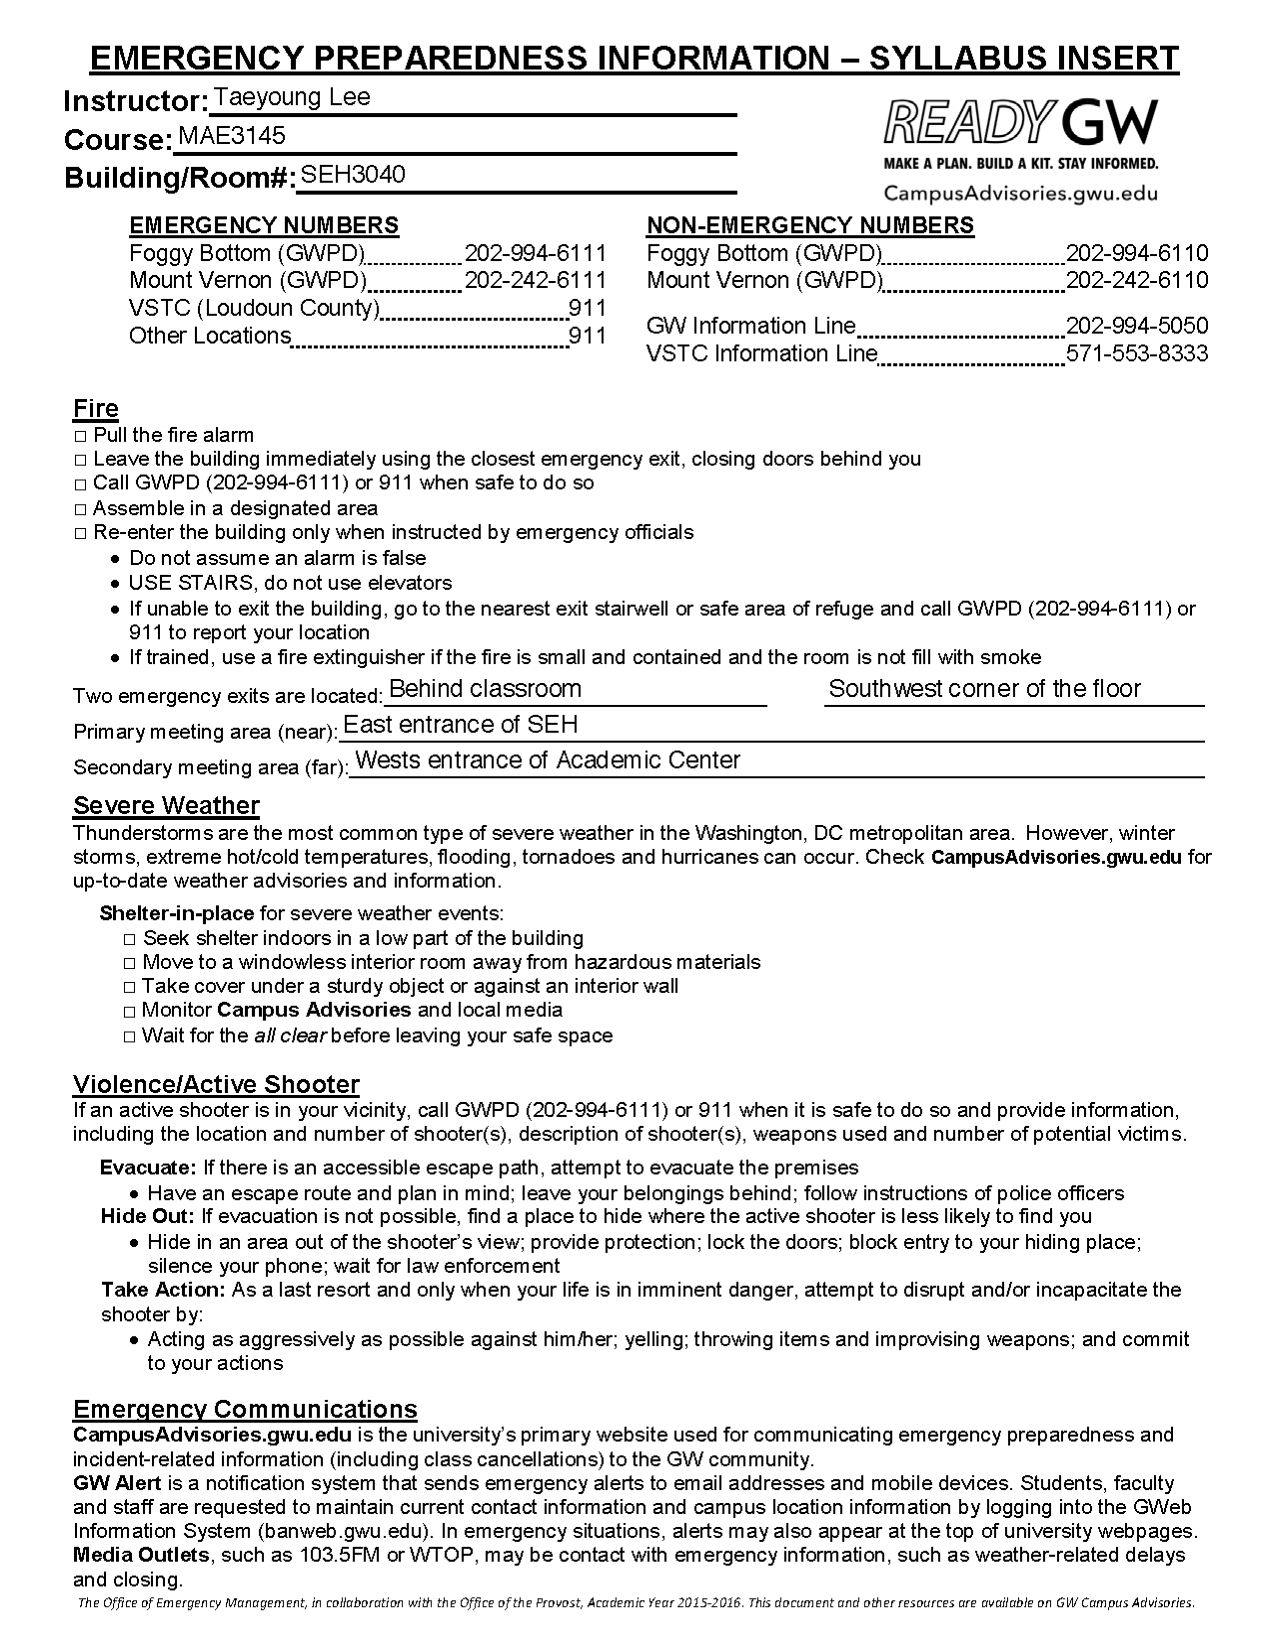
\includepdf{Syllabus_Insert_MAE3145_0}
\end{document}

